\section{Asymptotic Form of the FP Probability}
\label{sec:limitf}
We will derive a new and very simple approach to computing asymptotic form for the FP probability of BFs. The new derivation is based on \textit{partitioned Bloom Filters} (pBF) that are used frequently to carry out parallel query. Its principle is simple: the BF is divided into $k$ even partitions, and each hash function only acts on one of the partitions, respectively. %With this structure Using this method, there is a characteristic/regulation in the partitioned Bloom Filter: each partition of the Bloom Filter has at least one 1, thus its entropy is not the maximum.
The probability that one bit of the BF array remains 0 after inserting $n$ elements in the BF becomes
\begin{equation}
p'_{partition} = \left( 1-\dfrac{k}{m} \right)^n
\label{equ:p'pBF}
\end{equation}
as now each hash maps into $\frac{m}{k}$ separate bits.

It is intuitive that the FP probability of partitioned BF is a littler bigger than that of BF. Unfortunately, there is no strict proof. Here we show one proof method, which is based on the following Lemma. 

\textbf{Lemma II:} For $m > 1 \;\;,   k >1, \;\; n > 1, \: m>k$,
\begin{equation}
\label{theorem1}
\left( 1-\dfrac{k}{m} \right)  ^n <
\left( 1-\dfrac{1}{m} \right)  ^{kn}
\end{equation}

A similar but different inequality is shown in page 3 of the well known BF survey \cite{BFSurvey}. The survey did not give the proof, thus we give one here.

\begin{proof}
Let $g(k)=( 1-\frac{1}{m} )  ^k- ( 1-\frac{k}{m} )$. For $k>1$, $g(k)$ is a continuous and derivable function and its derivative is:
\begin{equation}
%g'(k)=k\left( 1- \dfrac{1}{m}\right) ^{k-1} +\dfrac{1}{m}
g'(k)=\left( 1- \dfrac{1}{m}\right)^k \ln\left(1-\dfrac{1}{m}\right)+\dfrac{1}{m}
\end{equation}
Since $m > 1$, $k > 1$, based on the derivative, we have:
\begin{equation}
\begin{aligned}
%g'(k)=k\left( 1- \dfrac{1}{m}\right) ^{k-1} +\dfrac{1}{m}
g'(k) %&=\left( 1- \dfrac{1}{m}\right)^k \ln\left(1-\dfrac{1}{m}\right)+\dfrac{1}{m} \\
> \left( 1- \dfrac{1}{m}\right)\ln\left(1-\dfrac{1}{m}\right)+\dfrac{1}{m}
\end{aligned}
\end{equation}
Let $f(m)=\left( 1- \dfrac{1}{m}\right)\ln\left(1-\dfrac{1}{m}\right)+\dfrac{1}{m}$, we can find $f'(m) = \dfrac{1}{m^2} \ln\left(1-\dfrac{1}{m}\right)< 0$, meaning that the function $f(m)$ is strictly decreasing. When $m$ goes to infinity, we have $\lim\limits_{m \to \infty}  f(m) =  0$. Therefore, we know that $f(m) \geqslant 0$, and $g'(k) > f(m) \geqslant 0$, meaning that the function $g(k)$ is strictly increasing.
%$f(m) \geqslant f(2)=\dfrac{1}{2} - \dfrac{1}{2}\ln\left(\dfrac{1}{2}\right)$. 
We have therefore 
\begin{equation}
0<\left( 1-\dfrac{k}{m} \right)   <
\left( 1-\dfrac{1}{m} \right)  ^k
\end{equation}
or 
\begin{equation}
\left( 1-\dfrac{k}{m} \right) ^n   <
\left( 1-\dfrac{1}{m} \right)  ^{kn}
\end{equation}
\end{proof}

%Therefore, the $p'$ of partitioned BF is larger than the $p'$ of BF, this is correct.
%Then the survey says that based on this, the FP probability of partitioned BF is larger than that of BF.
%This derivation is not strict, because two reasons: 1) the FP probability of BF cannot be get by $p'$; 2) the hash mechanism of partitioned BF and BF are different. 
%Therefore, we cannot draw the conclusion that the FP probability of partitioned BF is large according to the above Lemma.


The above lemma shows that $p'_{partition} < p'_{true}$ or equivalently $1-p'_{partition} > 1-p'_{true}$. The probability that one bit of the array is set to 1 in a pBF of size $m$, and with $k$ hash functions is therefore larger than that of Bloom filter with same parameters, meaning that the pBF will in average have more bits set than the corresponding BF, and finally the FP probability of the pBF will be larger than that of the standard BF  $f_{true}$, \ie, $f_{partition} > f_{true}$. In addition, Christensen’s bounds in Eq. \ref{fBound} state that the precise value of FP probability for a BF $f_{true}$ is larger than $f_{bloom}$, \ie, $f_{true} > f_{bloom}$. Therefore, we have the following upper and lower bounds:
%%%%%%%%%%%%%%%%%%%%%%%%%%%%%%%%%%%%%%%%%By Qiaobin%%%%%%%%%%%%%%%%%%%%%%%%%%%%%%%

%Having characteristic means that the information entropy is not the maximum, thus the FP probability $f_{partition}$ is larger than the standard Bloom Filter  $f_{true}$, thus we get
%However, Christensen’s bounds in Eq. \ref{fBound} state that the precise value of FP probability for a BF $f_{true}$ is larger than $f_{bloom}$, meaning that


\begin{equation}
\label{bigbig}
f_{partition} > f_{true} > f_{bloom}
\end{equation}



For partitioned BF, the probability that one bit of the array is still 0 $p'$ is shown in Eq. \ref{equ:p'pBF}.
Different from standard Bloom Filter, for partitioned Bloom Filter, the event ``$E(h_1=1),E(h_2=1),E(h_3=1),...,E(h_{i-1}=1)$'' is independent with the event ``$E(h_{i-1}=1)$'', where $E(h_{i-1}=1)$ means the event that the position of $h_{i-1}(x)$ is 1, because each hash function is responsible for one partition, and has no effect with each other. Therefore, 

\begin{equation}
f_{partition}=(1-p'_{partition})^k=\left( 1- \left( 1-\dfrac{k}{m} \right)^n \right) ^k
\end{equation}

Then the formula~\ref{bigbig} becomes

\begin{equation}
\left( 1- \left( 1-\dfrac{k}{m} \right)^n \right) ^k > f_{true} > \left( 1- \left( 1-\dfrac{1}{m} \right)^{nk} \right) ^k
\end{equation}

Then we use the well known limit formula:

\begin{equation}
\lim\limits_{x \to \infty} \left( 1-\dfrac{1}{x}\right) ^{-x} = e
\end{equation}

%and then get

%%%%%%%%%%%%%%%%%%%%%%%%%%%%%%%%%%%%%%%%%By Qiaobin%%%%%%%%%%%%%%%%%%%%%%%%%%%%%%%
%One can easily derive the FP probability for pBF as:
%\begin{equation}
%f_{partition}=(1-p'_{partition})^k=\left( 1- \left( 1-\dfrac{k}{m} \right)^n \right) ^k
%\end{equation}
%Different from standard Bloom Filter, the second independence assumption (the independence between the value of positions mapped by different hash functions) is valid as each hash accesses a bit in a different partition, therefore the above formula is precise resulting in the below upper and lower bounds for $f_{true}$: 

%\emph{Note that the above formula is the correct form of the pBF's FP probability, since all the $k$ hashings access different bits in different partitions, which guarantees that all the $k$ queried bits are independent and satisfies the ``multiple principle''.}
%Therefore, the formula~\ref{bigbig} becomes
%\begin{equation}
%\left( 1- \left( 1-\dfrac{k}{m} \right)^n \right) ^k > f_{true} > \left( 1- \left( 1-\dfrac{1}{m} \right)^{nk} \right) ^k
%\end{equation}
%%%%%%%%%%%%%%%%%%%%%%%%%%%%%%%%%%%%%%%%%By Qiaobin%%%%%%%%%%%%%%%%%%%%%%%%%%%%%%%

Asymptotically when $m$ becomes large, we already know that $f_{bloom}$ converges to the term in Eq. \ref{fBloom}. Nevertheless, the upper bound has also an asymptotic behaviour as :
\begin{equation}
\label{flim}
%\begin{aligned}
\lim\limits_{m \to \infty} \left(1-\left(1-\frac{1}{m}\right)^{nk}\right)^k = \left(1-e^{-nk/m}\right)^k 
%\end{aligned}
\end{equation}
that is the same term as the lower bound limit. Through the Sandwich Theorem (also known as squeeze theorem) we get, similarly to Christensen and to Bose, that :
\begin{equation}
\label{flimtrue}
\lim\limits_{m \to \infty}  f_{true} =  \left(1-e^{-nk/m}\right)^k 
\end{equation}

This means that when $m$ is large, the Bloom's formula can be used with negligible error. However, we still need to evaluate what means \textit{$m$ being large}. We will do this by comparing the two bounds we have in hand: the one from Bose and the one we derived in this paper. 

\begin{figure}
\centering
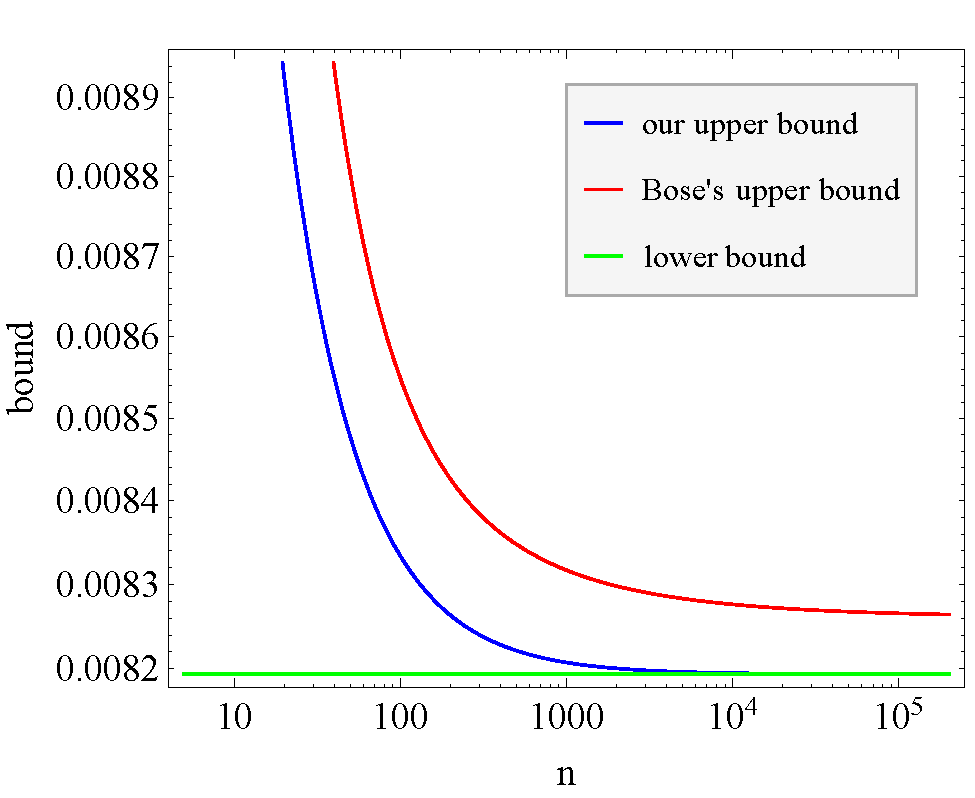
\includegraphics[width=\figwidth]{LogLog_lowerUpper}
\caption{Upper and lower bound for $f_{true}$ for $k=7$ and $m=10n$.}
\label{fig:uplowbound}
\end{figure}

We show in Figure~\ref{fig:uplowbound} the two upper bounds along with the lower bound obtained for $k=7$  and $m=10n$ as a function of $n$, the number of elements inserted in the BF. As can be seen, the upper bound derived in this paper and the lower bound $f_{bloom}$ converge relatively fast for $n=9$, while the upper bound derived by Bose has a much slower convergence. We can see this better by looking at the behavior of the bounds error ratio $\beta$, defined as $\beta=\frac{upper bound - lower bound}{lower bound}$, for the two bounds in Figure \ref{fig:ratio}.
\begin{figure}
\centering
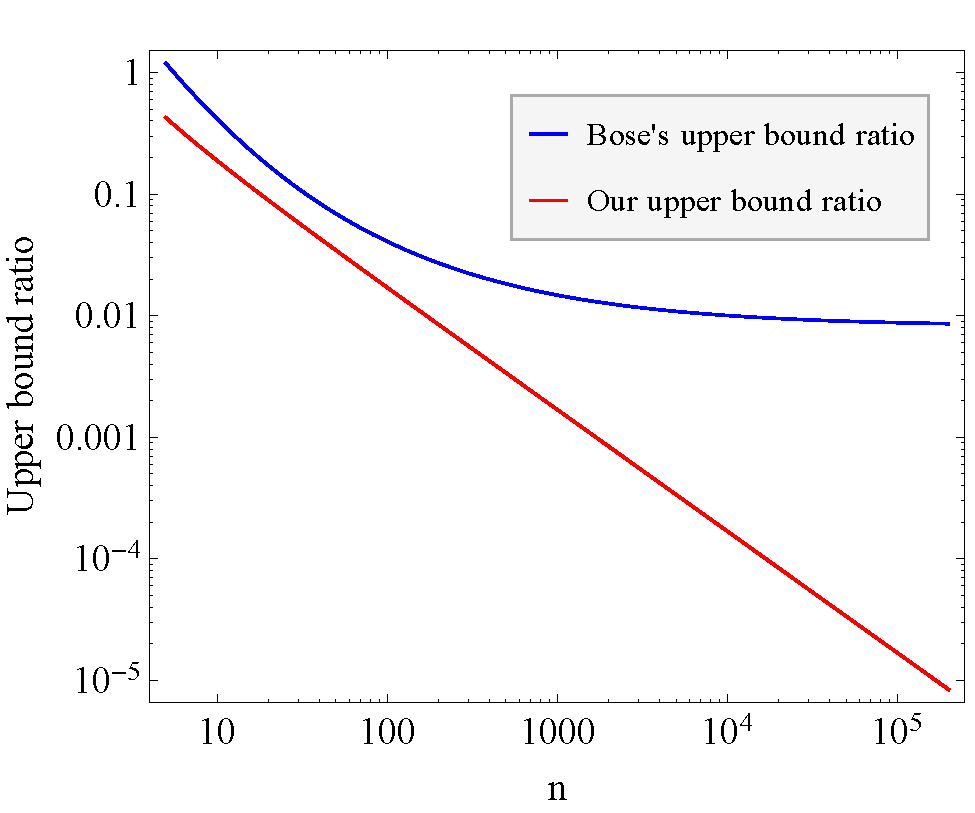
\includegraphics[width=\figwidth]{LogLog_ratio}
\caption{Bounds error ratio for Bose's bound and the bound derived in this paper for $k=7$ and $m=10n$. }
\label{fig:ratio}
\end{figure}
As can be seen, the gap between the our derived upper bound and $f_{bloom}$ is decreasing polynomially at a constant speed, while Bose bound has a lower speed of convergence. In order to extend this observation, we show in Figure \ref{fig:ratiok} the evolution of the bounds error ratio for a BF with $m=10000$, $n=1000$ and varying $k$. 
\begin{figure}
\centering
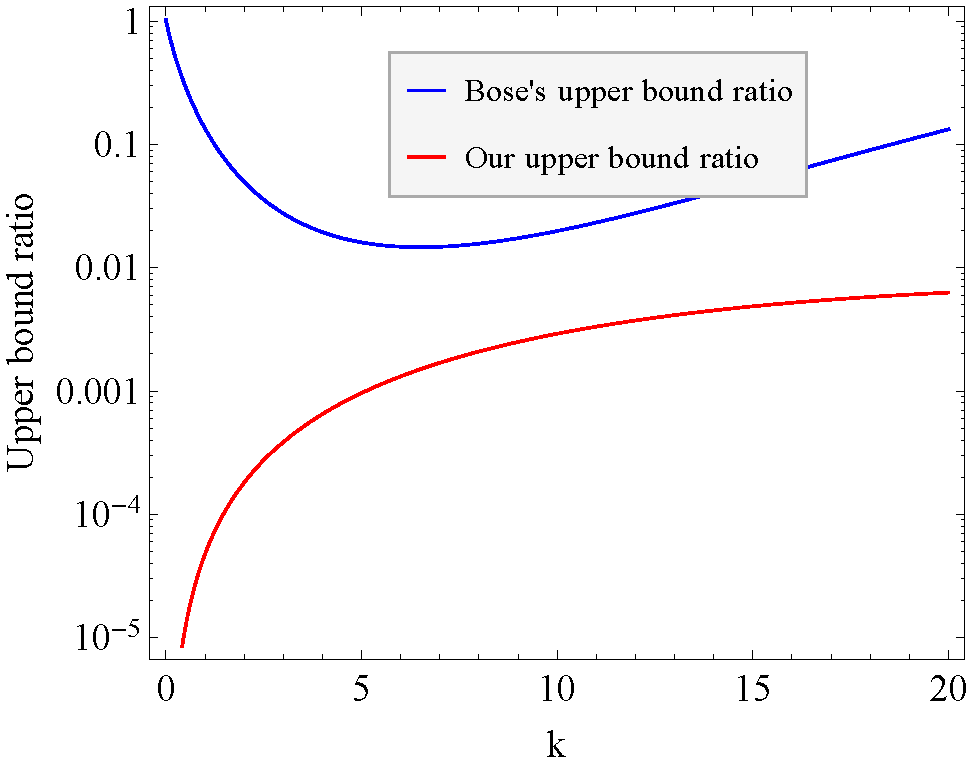
\includegraphics[width=\figwidth]{ratioLog_k}
\caption{Bounds error ratio for Bose's bound and the bound derived in this paper for $m=10000$, $n=1000$ and varying $k$.}
\label{fig:ratiok}
\end{figure}
As expected, error involved with using $f_{bloom}$ increases with the number of hash functions $k$ increases. However, it can be seen that the convergence behavior of the bounds derived in this paper is much better than the one obtained by Bose. 



 %\textbf{One Example.}
% \textbf{Example 1:}
%
% For example, $m=2, n=1, k=2$, the result using the Bloom's formula is 4.5/8.
% After hashing, there will be three cases: 10, 01, 11, thus the true false positive is 
%
% \begin{equation}
% \dfrac{1}{4}\times \dfrac{1}{4} +\dfrac{1}{4}\times \dfrac{1}{4} +1 \times \dfrac{2}{4}=\dfrac{5}{8}
% \end{equation} 
% In conclusion, the error of Bloom's formula is 1/16, when $m$ is 2.


% For example, $m=3, \, n=1,  \,  k=2$, there are three cases:
%
% Case I: two hashing map to the same position, the BF array will be one of the three: 100, 010, 001, each with the probability of 1/9. The FP probability of Case I is: 
%
% \begin{equation}
% (\dfrac{1}{3} \times \dfrac{1}{9} ) \times 3 = \dfrac{1}{9}
% \end{equation} 
% Case II: two hashings map to different positions, the BF array will be one of the three: 110, 101, 011, each with the probability of 2/9. First we compute the probability of no false positive:
%
% 1) Both the first and the second hashing positions are 0, the probability is 1/9.
%
% 2) The first hash position is 0, the second hash position is 1, the probability is 
% \begin{equation}
% \dfrac{1}{3} \times \dfrac{2}{3} = \dfrac{2}{9}
% \end{equation} 
%
% 3) The first hash position is 1, the second hash position is 0, the probability is also 2/9.
%
% Therefore, the probability of false positive of Case II is:
%
% \begin{equation}
% 1-\dfrac{1}{9}-\dfrac{2}{9}-\dfrac{2}{9}=\dfrac{4}{9}
% \end{equation}
%
% In sum, the probability of false positive of this example is:
%
%
% \begin{equation}
% \frac{1}{9}\times 3 \times \frac{1}{9}+ \frac{4}{9}\times 3\times \frac{2}{9}=\dfrac{27}{81}
% \end{equation}
%
% Note that the result using Bloom's formula is 25/81, and the error is 2/81.
%
%
%%套公式得出的结果是 25/81,误差是1/40.5
%%
%%\subsection{the results of suboptimal value}
%%For Standard Bloom Filter (SBF), the FP probability is given by:
%%
%%\begin{equation}
%%f=\left(1-\left(1-\dfrac{1}{m}\right)^{nk}\right)^k
%%\end{equation}
%%
%%When m is large, the formula reduces to
%%
%%\begin{equation}
%%\label{math:fpLargem}
%%f=\left(1-e^{-\dfrac{nk}{m}}
%%\right)^k
%%\end{equation} 